\section{Durchführung}
\label{sec:Durchführung}

% Was wurde gemessen bzw. welche Größen wurden variiert?
Die folgenden Messvorgänge werden für je zwei Stäbe verschiedener Querschnitte (rund und quadratisch) und verschiedener Materialien durchgeführt.

Bevor die Durchbiegung eines Stabes gemessen wird, ist es sinnvoll die Maße dessen zu messen.
Zunächst wird also die Länge des Stabes mithilfe eines Maßbands gemessen und die Masse mithilfe einer elektrischen Waage gemessen.
Da der Stab eventuell Unregelmäßigkeiten in seiner Breite bzw. seinem Durchmesser vorweist, muss sowohl die Breite als auch den Durchmesser an mehreren Stellen mithilfe eines Messschiebers gemessen werden, um später daraus einen Mittelwert zu bilden.

Außerdem muss darauf geachtet werden, dass die $\SI{0.01}{\milli\meter}$ Skalen der Messuhren vor dem Messen auf Null gesetzt werden, damit diese Skala richtig abgelesen werden kann.

\subsection{Messung der Durchbiegung eines einseitig eingespannten Stabes}
\label{sec:Durchführung_Einseitig}

\begin{figure}
    \centering
    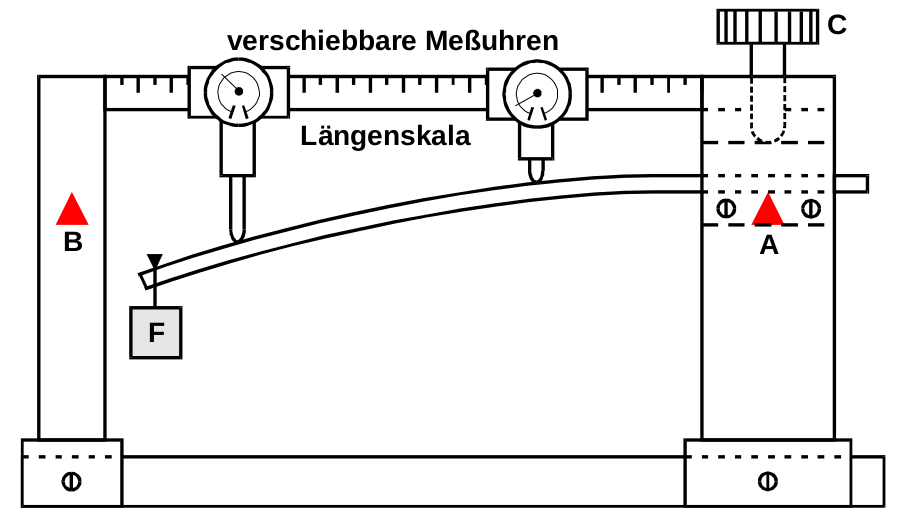
\includegraphics[width=\textwidth]{images/skizze_6.png}
    \caption{Versuchsaufbau zum Messen der Durchbiegung\cite{V103}}
    \label{fig:skizze_6}
\end{figure}

Der zu vermessende Stab wird in die Messvorrichtung, wie in \autoref{fig:skizze_6} ohne angehangenes Gewicht einseitig eingespannt.
Die Länge des Stabes wird vom Einspannungsort aus gemessen.
Nun wird die Messuhr an 15 verschiedene Stellen des Stabes geschoben und die Auslenkung an dieser Stelle wird abgelesen. Zusätzlich muss notiert werden, an welchem Abstand zum Einspannungsort die Auslenkung abgelesen wurde.
Dies wird vorerst ohne angehangenes Gewicht gemessen, da nicht davon ausgegangen werden kann, dass der zu vermessende Stab perfekt gerade ist.

Es wird dann ein Gewicht gesucht, welches mithilfe einer Aufhängung an das Ende des Stabes gehangen wird und dort eine Durchbiegung des Stabes zwischen $\num{3}$ und $\SI{7}{\milli\meter}$ verursacht.
Die Masse dieses Gewichts wird mithilfe einer Waage gemessen, wobei beachtet werden muss, dass die Masse der Aufhängung zusätzlich gemessen werden muss.
Nun wird wie zuvor die Auslenkung des Stabes an den gleichen 15 Stellen gemessen, allerdings ist diesmal der Stab durch das angehangene Gewicht durchgebogen. 

\subsection{Messung der Durchbiegung eines beidseitig eingespannten Stabes}
\label{sec:Durchführung_Beidseitig}

Um die Durchbiegung eines Stabes zu messen, welcher beidseitig, also an den Punkten A und B in \autoref{fig:skizze_6}, eingespannt ist, muss dieser zunächst wie beim einseitigen Einspannen ohne angehangenes Gewicht vermessen werden. Zuerst muss also der Abstand von den Einspannungsorten gemessen werden.
Danach wird mit den Messuhren auf jeder Hälfte die Auslenkung an 10 Stellen gemessen.
Hier muss darauf geachtet werden, dass für jede Hälfte des Stabes eine andere Messuhr verwendet wird.

Dann wird der Stab erneut beidseitig eingespannt, allerdings wird nun ein Gewicht in die Mitte des Stabes gehangen, das so schwer ist, dass eine Durchbiegung gemessen werden kann. 
Dieses Gewicht muss wieder mit einer Waage vermessen werden.
Mit diesem angehangenen Gewicht werden die Auslenkungen der Messuhr wieder an den zuvor gemessenen Stellen abgelesen.

